% rubber: shell_escape
\synctex=1
\documentclass[11pt,aspectratio=169]{beamer}

\usepackage[T1]{fontenc}
\usepackage[english]{babel}
\usepackage{amsmath,amssymb,amsfonts}
\usepackage{mathtools}
\usepackage{bm}
\usepackage{tikz}
\usetikzlibrary{arrows.meta,positioning,shapes,calc}
\usepackage{pgfplots}
\usepgfplotslibrary{statistics,groupplots}
\usepackage{xcolor}
\usepackage{booktabs}
\pgfplotsset{compat=1.18}

\usefonttheme[onlymath]{serif}

\definecolor{darkblue}{RGB}{0,51,102}
\definecolor{lightblue}{RGB}{230,240,250}
\definecolor{darkgreen}{RGB}{0,102,51}
\definecolor{darkred}{RGB}{153,0,0}
\definecolor{orange}{RGB}{255,128,0}
\definecolor{violet}{RGB}{102,0,153}
\definecolor{lightgreen}{RGB}{220,245,220}
\definecolor{lightorange}{RGB}{255,240,220}
\definecolor{gray}{gray}{0.4}

\newcommand{\E}{\mathbb{E}}
\newcommand{\V}{\mathbb{V}}
\newcommand{\PP}{\mathbb{P}}
\newcommand{\code}[1]{\texttt{#1}}

% Git hashes: this repository, and the commit of the accuracy branch of Dynare
% that produced the results (written by mod/run_example.m).
\usepackage{xstring}
\usepackage{catchfile}
\immediate\write18{git rev-parse --short HEAD > git.hash 2>/dev/null || echo uncommitted > git.hash}
\CatchFileDef{\HEAD}{git.hash}{\endlinechar=-1}
\newcommand{\gitrevision}{\StrLeft{\HEAD}{11}}
\IfFileExists{../mod/results/dynare.hash}{\CatchFileDef{\DYNAREHEAD}{../mod/results/dynare.hash}{\endlinechar=-1}}{\def\DYNAREHEAD{unknown}}

\usepackage{ccicons}

\setbeamertemplate{footline}{
  \hfill\vspace*{1pt}\cczero\enspace\gitrevision\enspace(dynare@\DYNAREHEAD)\enspace--\enspace\insertframenumber/\inserttotalframenumber\enspace--\enspace\today\enspace}

\setbeamertemplate{navigation symbols}{}

% Results produced by the examples in ../mod.
\newcommand{\growthDetResid}{0}
\newcommand{\growthSSResid}{1.45\times10^{-5}}
\newcommand{\growthSSGapThree}{1.11\times10^{-13}}
\newcommand{\growthSSGapFive}{1.51\times10^{-17}}
\newcommand{\growthSSGapNine}{8.22\times10^{-18}}
\newcommand{\growthSSResidSmall}{1.45\times10^{-7}}
\newcommand{\growthSSRatio}{100.0}
\newcommand{\growthSSUnits}{3.998\times10^{-3}}
\newcommand{\growthSSNewton}{3.992\times10^{-3}}
\newcommand{\growthGapMean}{0}
\newcommand{\growthGapQuad}{1.85\times10^{-7}}
\newcommand{\growthBudgetNewtonK}{-1.60}
\newcommand{\growthNewtonGap}{3.68\times10^{-16}}
\newcommand{\growthSSc}{2.75}
\newcommand{\growthSSk}{38}
\newcommand{\growthBudgetUnitsK}{-1.59}
\newcommand{\growthUnitsMean}{1.44\times10^{-2}}
\newcommand{\growthUnitsMax}{8.88\times10^{-2}}
\newcommand{\growthNewtonCMean}{1.42\times10^{-2}}
\newcommand{\growthNewtonCMax}{9.77\times10^{-2}}
\newcommand{\growthUnitsMeanLog}{-1.84}
\newcommand{\growthUnitsMaxLog}{-1.05}
\newcommand{\growthNewtonCMeanLog}{-1.85}
\newcommand{\growthNewtonCMaxLog}{-1.01}
\newcommand{\growthSimPoints}{1000}
\newcommand{\growthGridPoints}{500}
\newcommand{\growthIrfPoints}{40}
\newcommand{\growthGridKlo}{29.91}
\newcommand{\growthGridKhi}{45.53}
\newcommand{\growthGridAlo}{-0.152}
\newcommand{\growthGridAhi}{0.152}

\newcommand{\linearMaxSim}{3.65\times10^{-15}}
\newcommand{\linearNSim}{200}
\newcommand{\linearMaxGrid}{3.25\times10^{-15}}
\newcommand{\linearNGrid}{200}
\newcommand{\linearMaxIrf}{1.02\times10^{-15}}
\newcommand{\linearNIrf}{40}

\newcommand{\burnsideExactFive}{1.81\times10^{-9}}
\newcommand{\burnsideExactEleven}{2.91\times10^{-15}}
\newcommand{\burnsideExactTwentyOne}{2.28\times10^{-15}}
\newcommand{\burnsideOrderOne}{2.29\times10^{-1}}
\newcommand{\burnsideOrderTwo}{1.59\times10^{-1}}
\newcommand{\burnsideOrderThree}{4.70\times10^{-2}}
\newcommand{\burnsideOrderFour}{3.25\times10^{-2}}
\newcommand{\burnsideNewtonOne}{5.9}
\newcommand{\burnsideNewtonFour}{0.8}
\newcommand{\burnsideDecades}{13.2}
\newcommand{\burnsideSteadyY}{3.86}

\newcommand{\dhmDf}{2}
\newcommand{\dhmInstruments}{constant and 1 lag(s) of the 1 normalized states}
\newcommand{\dhmMeanExact}{2.15}
\newcommand{\dhmLowerExact}{0.010}
\newcommand{\dhmUpperExact}{0.035}
\newcommand{\dhmMeanOne}{23.10}
\newcommand{\dhmLowerOne}{0.000}
\newcommand{\dhmUpperOne}{0.995}
\newcommand{\dhmMeanTwo}{3.87}
\newcommand{\dhmLowerTwo}{0.005}
\newcommand{\dhmUpperTwo}{0.130}
\newcommand{\dhmInstrumentsReplic}{200}

\newcommand{\epBurnsidePoints}{20}
\newcommand{\epbFailures}{0}
\newcommand{\epbDet}{2.12\times10^{-1}}
\newcommand{\epbSEPone}{1.75\times10^{-1}}
\newcommand{\epbSEPoneHtwo}{3.72\times10^{-2}}
\newcommand{\epbSEPoneHfour}{1.42\times10^{-2}}
\newcommand{\epbSEPtwo}{1.46\times10^{-1}}
\newcommand{\epbSEPtwoHfour}{5.97\times10^{-3}}
\newcommand{\epbSEPthree}{1.22\times10^{-1}}
\newcommand{\epbPertFour}{2.86\times10^{-2}}

\newcommand{\irrNewtonOccI}{0.40}
\newcommand{\irrNewtonEPI}{0.03}
\newcommand{\irrByEqOccCEuler}{0.03}
\newcommand{\irrByEqOccCBudget}{0.13}
\newcommand{\irrByEqOccCInvdef}{0.16}
\newcommand{\irrByEqOccCTotal}{0.08}
\newcommand{\irrByEqMeanRatioMin}{1}
\newcommand{\irrByEqMeanRatioMax}{3}
\newcommand{\irrByEqMaxRatioMin}{3}
\newcommand{\irrByEqMaxRatioMax}{7}
\newcommand{\irrHybridGain}{0.8}
\newcommand{\irrPoints}{200}
\newcommand{\irrNodes}{5}
\newcommand{\irrBinding}{79}
\newcommand{\irrFloor}{-2.53}
\newcommand{\irrCrossCheck}{0}
\newcommand{\irrFailures}{0}
\newcommand{\irrElapsed}{39}
\newcommand{\irrEulerEP}{1.56\times10^{-4}}
\newcommand{\irrEulerMeanEP}{9.88\times10^{-5}}
\newcommand{\irrEulerSEP}{1.26\times10^{-4}}
\newcommand{\irrEulerMeanSEP}{8.52\times10^{-5}}
\newcommand{\irrEulerSEPhTwo}{6.04\times10^{-5}}
\newcommand{\irrEulerMeanSEPhTwo}{2.79\times10^{-5}}
\newcommand{\irrEulerSEPhFour}{6.05\times10^{-5}}
\newcommand{\irrEulerMeanSEPhFour}{2.79\times10^{-5}}
\newcommand{\irrEulerOccBin}{4.34\times10^{-3}}
\newcommand{\irrEulerMeanOccBin}{3.74\times10^{-4}}
\newcommand{\irrRatioOccEP}{27.8}
\newcommand{\irrRatioMeanOccEP}{3.8}
\newcommand{\irrRatioEPSEP}{1.2}
\newcommand{\irrRatioEPSEPhTwo}{3.5}
\newcommand{\irrRatioEPSEPhFour}{3.5}
\newcommand{\irrRatioMaxEPSEPhFour}{2.6}
\newcommand{\irrDistOccI}{0.41}
\newcommand{\irrDistSepI}{0.02}
\newcommand{\irrDistSepHFourI}{0.11}

\newcommand{\sweepPoints}{60}
\newcommand{\sweepElapsed}{297}
\newcommand{\sweepFailures}{3}
\newcommand{\sweepSigmaMax}{0.03}
\newcommand{\sweepOccGapTwo}{0.5}
\newcommand{\sweepHybridGainTwo}{0.5}
\newcommand{\sweepOccGapFive}{0.2}
\newcommand{\sweepHybridGainFive}{0.3}

\newcommand{\bsPoints}{200}
\newcommand{\bsBurn}{1000}
\newcommand{\bsEgmIterations}{229}
\newcommand{\bsEgmNodes}{81}
\newcommand{\bsQuadFloorMax}{-3.3}
\newcommand{\bsQuadFloorMean}{-4.1}
\newcommand{\bsGapMin}{1.5}
\newcommand{\bsGapMax}{2.1}
\newcommand{\bsEgmTime}{176}
\newcommand{\bsElapsed}{1168}
\newcommand{\bsElapsedSim}{159}
\newcommand{\bsTsim}{500}
\newcommand{\bsFailures}{0}
\newcommand{\bsEulerEP}{2.33\times10^{-2}}
\newcommand{\bsEulerMeanEP}{8.95\times10^{-3}}
\newcommand{\bsBufferEP}{0.09}
\newcommand{\bsAtLimitEP}{37}
\newcommand{\bsEulerSEP}{9.45\times10^{-3}}
\newcommand{\bsEulerMeanSEP}{4.52\times10^{-3}}
\newcommand{\bsBufferSEP}{0.10}
\newcommand{\bsAtLimitSEP}{26}
\newcommand{\bsEulerSEPhTwo}{9.45\times10^{-3}}
\newcommand{\bsEulerMeanSEPhTwo}{4.52\times10^{-3}}
\newcommand{\bsBufferSEPhTwo}{0.10}
\newcommand{\bsAtLimitSEPhTwo}{26}
\newcommand{\bsEulerSEPhFour}{9.45\times10^{-3}}
\newcommand{\bsEulerMeanSEPhFour}{4.52\times10^{-3}}
\newcommand{\bsBufferSEPhFour}{0.10}
\newcommand{\bsAtLimitSEPhFour}{26}
\newcommand{\bsEulerSEPoTwo}{5.99\times10^{-3}}
\newcommand{\bsEulerMeanSEPoTwo}{3.23\times10^{-3}}
\newcommand{\bsBufferSEPoTwo}{0.12}
\newcommand{\bsAtLimitSEPoTwo}{22}
\newcommand{\bsEulerSEPoThree}{5.79\times10^{-3}}
\newcommand{\bsEulerMeanSEPoThree}{2.44\times10^{-3}}
\newcommand{\bsBufferSEPoThree}{0.13}
\newcommand{\bsAtLimitSEPoThree}{21}
\newcommand{\bsEulerOccBin}{1.72\times10^{-1}}
\newcommand{\bsEulerMeanOccBin}{1.08\times10^{-2}}
\newcommand{\bsBufferOccBin}{0.09}
\newcommand{\bsAtLimitOccBin}{36}
\newcommand{\bsEulerEGM}{5.47\times10^{-4}}
\newcommand{\bsEulerMeanEGM}{8.58\times10^{-5}}
\newcommand{\bsBufferEGM}{0.18}
\newcommand{\bsAtLimitEGM}{17}


\pgfplotsset{
  every axis/.append style={font=\footnotesize, grid=major, grid style={gray!25}},
  table/col sep=comma
}

\title{Measuring the accuracy of solutions in Dynare}
\subtitle{The \code{accuracy} branch: strategies, examples, and extended path versus OccBin}
\author{}
\date{}
\institute{}

\AtBeginSection[]
{
  \begin{frame}
    \frametitle{Outline}
    \tableofcontents[currentsection]
  \end{frame}
}

\begin{document}

\begin{frame}
\titlepage
\end{frame}

\begin{frame}{Outline}
\tableofcontents
\end{frame}

%==============================================================================
\section{Motivation and principle}
%==============================================================================

\begin{frame}{Motivation -- What was missing}

\begin{itemize}

\item Dynare computes solutions by \textbf{perturbation} (orders 1 to $k$, with or without pruning), by \textbf{extended path} (deterministic or stochastic) and by \textbf{OccBin} (piecewise linear), but offered \textbf{no way} of measuring how accurate they are.\newline

\item The new package \code{matlab/+accuracy/} answers two questions, \textbf{whatever the method} that produced the solution:\newline
  \begin{itemize}

  \item how far is a solution from satisfying the model?\newline

  \item how do two solutions of the same economy compare, when they come from different \code{.mod} files?

  \end{itemize}

\end{itemize}

\end{frame}

\begin{frame}{Principle -- Residuals under the expectation}

\begin{itemize}

\item The model is $\E_t\left[f(y_{t-1}, y_t, y_{t+1}, u_t;\theta)\right] = 0$ and a solution is a decision rule $y_t = g(y_{t-1}, u_t)$.\newline

\item At an evaluation point $(y_{t-1}, u_t)$, the residual is the expectation over next period innovations, computed by quadrature:
  \[
  \boxed{R = \sum_{j=1}^{J}\omega_j\, f\Big(y_{t-1},\ y_t,\ g\big(y_t, \varepsilon^{(j)}\big),\ u_t;\theta\Big),\qquad y_t = g(y_{t-1},u_t)}
  \]
  With the exact $g$ and an exact quadrature, $R=0$.\newline

\item Three sources of error show up in $R$, and the tools are designed to tell them apart: the \textbf{approximation} of $g$ (what we want to measure), the \textbf{quadrature} ($J$ nodes), and the \textbf{solver} when $g$ is itself the output of a numerical solve (extended path, OccBin).

\end{itemize}

\end{frame}

\begin{frame}{Principle -- Strategies covered}

\begin{center}
    \small
    \renewcommand{\arraystretch}{1.3}
    \begin{tabular}{lll}
        \toprule
        Strategy & What it measures & Cost \\
        \midrule
        Residuals by quadrature & $\E_t f$ at chosen points & $J$ evaluations of $g$ per point \\
        Newton normalization & implied error on each $y_t$ & one linear solve per point \\
        Units of a variable & error in units of, e.g., $c$ & one scalar root per point \\
        Exact solution & the quadrature error alone & needs a closed form \\
        Den Haan--Marcet & orthogonality of realized errors & one evaluation per period \\
        Comparison & common equations, distance & as above, per method \\
        \bottomrule
    \end{tabular}
\end{center}

All the numbers in these slides are produced by the \code{.mod} files of \code{./mod}, run with \code{make results}.

\end{frame}

%==============================================================================
\section{Architecture}
%==============================================================================

\begin{frame}[fragile]{Architecture -- Entry point}

\begin{itemize}

\item No new preprocessor command: a MATLAB call after \code{stoch\_simul}, in the \code{.mod} file.

 \medskip
  
\begin{semiverbatim}\footnotesize
stoch_simul(order=2, periods=0, irf=0);
oo_ = accuracy.check(M_, options_, oo_, 'points', \{'simulation','grid'\}, ...
                     'quadrature_nodes', 7, 'seed', 1);
\end{semiverbatim}

\medskip
 
\item Options as name/value pairs or a structure; an \textbf{unknown option is an error}, so that a typo cannot silently leave a default in place.\newline

\item Results in \code{oo\_.accuracy}: one field per kind of points (\code{residuals}, \code{newton}, \code{units}, \code{regimes}, \code{eval\_failures}, \dots), plus \code{equations}, \code{nodes}, \code{dhm}.

\end{itemize}

\end{frame}

\begin{frame}{Architecture -- What \code{accuracy.check} does}

\begin{center}
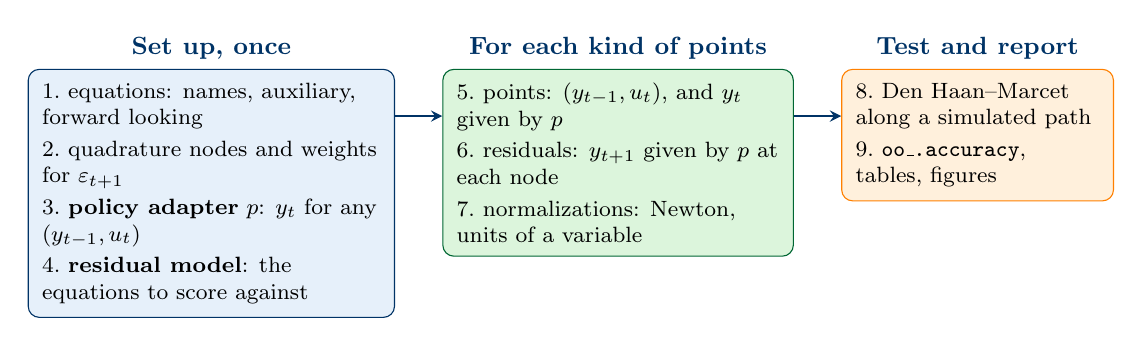
\begin{tikzpicture}[
  phase/.style={rectangle, draw=darkblue, fill=lightblue, text width=4.3cm, align=flush left, anchor=north, rounded corners,
                inner sep=5pt, font=\footnotesize},
  loop/.style={rectangle, draw=darkgreen, fill=lightgreen, text width=4.1cm, align=flush left, anchor=north, rounded corners,
               inner sep=5pt, font=\footnotesize},
  report/.style={rectangle, draw=orange, fill=lightorange, text width=3.1cm, align=flush left, anchor=north, rounded corners,
              inner sep=5pt, font=\footnotesize},
  head/.style={font=\small\bfseries, text=darkblue},
  arrow/.style={->, >=stealth, thick, darkblue}]
  \node[phase] (setup) at (0,0) {
    1.~equations: names, auxiliary, forward looking\\[2pt]
    2.~quadrature nodes and weights for $\varepsilon_{t+1}$\\[2pt]
    3.~\textbf{policy adapter} $p$: $y_t$ for any $(y_{t-1},u_t)$\\[2pt]
    4.~\textbf{residual model}: the equations to score against};
  \node[loop, anchor=north west] (points) at ($(setup.north east)+(0.6cm,0)$) {
    5.~points: $(y_{t-1},u_t)$, and $y_t$ given by $p$\\[2pt]
    6.~residuals: $y_{t+1}$ given by $p$ at each node\\[2pt]
    7.~normalizations: Newton, units of a variable};
  \node[report, anchor=north west] (report) at ($(points.north east)+(0.6cm,0)$) {
    8.~Den Haan--Marcet along a simulated path\\[2pt]
    9.~\code{oo\_.accuracy}, tables, figures};
  \node[head, anchor=south] at (setup.north) {Set up, once};
  \node[head, anchor=south] at (points.north) {For each kind of points};
  \node[head, anchor=south] at (report.north) {Test and report};
  \draw[arrow] ($(setup.north east)+(0,-0.6)$) -- ($(points.north west)+(0,-0.6)$);
  \draw[arrow] ($(points.north east)+(0,-0.6)$) -- ($(report.north west)+(0,-0.6)$);
\end{tikzpicture}
\end{center}

\begin{itemize}

\item The two pieces that do the work are built in the set up: the adapter $p$ hides how the solution was obtained, the residual model says which equations it must satisfy.\newline

\item The kinds of points are those of the \code{points} option: \code{'simulation'}, \code{'grid'}, \code{'irf'}.

\end{itemize}

\end{frame}

\begin{frame}{Architecture -- Model options}

The residuals come from the dynamic model files, \code{+fname/dynamic\_resid} and \code{dynamic\_g1} (M-files, or MEX with \code{use\_dll}), which are written in \textbf{levels}.\newline

\begin{itemize}

\item \code{loglinear} is \textbf{refused}: \code{oo\_.dr} then holds a decision rule for $\log y$, while the equations are in levels. Supporting it would mean exponentiating every adapter's output and applying the chain rule in the Newton and units normalizations.\newline

\item \code{bytecode} and \code{block} are \textbf{accepted}: the preprocessor writes the plain dynamic files whatever the options.\newline

\item Also refused: grid points under pruning, pruned decision rules in \code{accuracy.compare} (the pruned state is not a function of the current state).

\end{itemize}

\end{frame}

\begin{frame}{Architecture -- The policy adapter}

\begin{center}
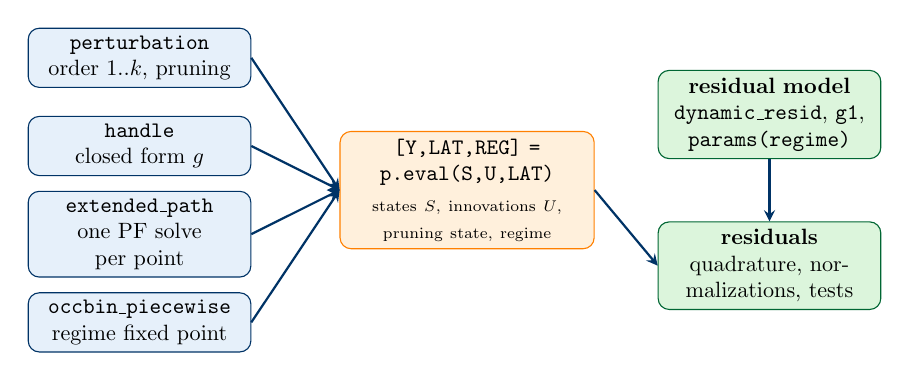
\begin{tikzpicture}[scale=0.8, transform shape,
  box/.style={rectangle, draw=darkblue, fill=lightblue, text width=3.3cm, align=center, minimum height=0.9cm, rounded corners},
  ok/.style={rectangle, draw=darkgreen, fill=lightgreen, text width=3.3cm, align=center, minimum height=0.9cm, rounded corners},
  alt/.style={rectangle, draw=orange, fill=lightorange, text width=3.8cm, align=center, minimum height=0.9cm, rounded corners},
  arrow/.style={->, >=stealth, thick, darkblue}]
  \node[box] (pert) at (0,3.3) {\code{perturbation}\\ order 1..$k$, pruning};
  \node[box] (hdl) at (0,1.9) {\code{handle}\\ closed form $g$};
  \node[box] (ep) at (0,0.5) {\code{extended\_path}\\ one PF solve per point};
  \node[box] (occ) at (0,-0.9) {\code{occbin\_piecewise}\\ regime fixed point};
  \node[alt] (p) at (5.2,1.2) {\code{[Y,LAT,REG] = p.eval(S,U,LAT)}\\[2pt] \scriptsize states $S$, innovations $U$, pruning state, regime};
  \node[ok] (rm) at (10,2.4) {\textbf{residual model}\\ \code{dynamic\_resid}, \code{g1}, \code{params(regime)}};
  \node[ok] (res) at (10,0) {\textbf{residuals}\\ quadrature, normalizations, tests};
  \draw[arrow] (pert.east) -- (p.west);
  \draw[arrow] (hdl.east) -- (p.west);
  \draw[arrow] (ep.east) -- (p.west);
  \draw[arrow] (occ.east) -- (p.west);
  \draw[arrow] (p.east) -- (res.west);
  \draw[arrow] (rm.south) -- (res.north);
\end{tikzpicture}
\end{center}

\begin{itemize}

\item The adapter hides the method: it evaluates the decision rule at an arbitrary state, and declares its \code{order}, the kinds of points it \code{supports} and a \code{cost\_hint} setting the default number of points.\newline

\item The \textbf{residual model} is kept distinct from the model that produced the decision rule (next slide).

\end{itemize}

\end{frame}

\begin{frame}[fragile]{Architecture -- Why a separate residual model}

\begin{itemize}

\item The same economy may have to be \textbf{written twice}, e.g.\ irreversible investment:
\begin{columns}[T]
\begin{column}{0.47\textwidth}
\begin{semiverbatim}\scriptsize
// OccBin: two regimes
[name='investment', bind='IRR']
i = ibar;
[name='investment', relax='IRR']
lambda = 0;
occbin_constraints; ... end;
\end{semiverbatim}
\end{column}
\begin{column}{0.47\textwidth}
\begin{semiverbatim}\scriptsize
// extended path: one equation
min(lambda, i - ibar) = 0;
// or, with an MCP solver
lambda = 0 _|_ i > ibar;
\end{semiverbatim}
\end{column}
\end{columns}

\medskip

\item OccBin only reads \code{occbin\_constraints}, which \code{extended\_path} refuses in the same file; $\perp$ is only read by the complementarity solvers $\Rightarrow$ two \code{.mod} files, each with its own equations.\newline

\item Both decision rules are scored against \textbf{one} set of equations, by default the \code{min} formulation. Not the $\perp$ one (not yet working when evaluating accuracy).\newline

\item \code{accuracy.map\_context} pairs variables by name and equations by \code{name} tag, whatever their order, and checks that variables, innovations and steady state agree.

\end{itemize}

\end{frame}

\begin{frame}{Architecture -- The four adapters}

\begin{center}
    \small
    \renewcommand{\arraystretch}{1.3}
    \begin{tabular}{llcr}
        \toprule
        Adapter & $g$ evaluated by & grid & cost \\
        \midrule
        \code{perturbation} & \code{local\_state\_space\_iteration\_*} & no pruning & 1 \\
        \code{handle} & user function \code{Y = f(S,U)} & yes & 1 \\
        \code{extended\_path} & \code{extended\_path\_core} & yes & $10^4$ \\
        \code{occbin\_piecewise} & \code{occbin.solver} & yes & $10^3$ \\
        \bottomrule
    \end{tabular}
\end{center}

\medskip

\begin{itemize}

\item The \textbf{order} only makes sense for perturbation; \code{accuracy.solution\_order} reproduces the silent fallback to order 1 when the Hessian is zero.\newline

\item The extended path is governed by its \textbf{stochastic order} (depth of the tree), hybrid correction, horizon and tolerance; OccBin by its horizon, on a first order solution. Reported in \code{oo\_.accuracy.solver}.\newline

\item \code{accuracy.simulate}: \code{simult\_} plus the latent state of pruning.

\end{itemize}

\end{frame}

%==============================================================================
\section{Residuals by quadrature}
%==============================================================================

\begin{frame}{Quadrature -- Filling the arguments of $f$}

\begin{itemize}

\item The expectation is taken over the innovations of $t+1$ only; $u_t$ belongs to the evaluation point.\newline

\item A state, in Dynare, is any variable that appears with a lag: with habits, $c_{t-1}$ enters the Euler equation, so $c$ is a state and $c_{t-1}$ is part of the evaluation point. The other variables, static or purely forward looking ($c$ without habits), never appear lagged: their lagged values, required by \code{dynamic\_resid} but never read, can be anything; the steady state is a placeholder.\newline

\item Auxiliary equations that any approximation satisfies exactly (lags, \code{diff}) are hidden, with a warning if their residual is not at machine precision. Substitutions of leads, expectations and logs carry a genuine error and are reported.\newline

\item Parameters are an argument of the residual model, \code{rm.params(regime)}: OccBin selects the equations of a regime through them.

\end{itemize}

\end{frame}

\begin{frame}{Quadrature -- Quadrature rules}

\begin{center}
    \small
    \renewcommand{\arraystretch}{1.1}
    \begin{tabular}{llc}
        \toprule
        \code{integration} & Construction & Nodes ($n$ shocks) \\
        \midrule
        \code{Tensor-Gaussian-Quadrature} & Gauss--Hermite, $m$ nodes & $m^n$ \\
        \code{Stroud-Cubature-3} & degree 3 monomial rule & $2n$ \\
        \code{Stroud-Cubature-5} & degree 5 monomial rule & $2n^2+1$ \\
        \code{Unscented} & sigma points & $2n+1$ \\
        \code{Deterministic} (new) & $\varepsilon_{t+1}=0$, weight 1 & $1$ \\
        \bottomrule
    \end{tabular}
\end{center}

\begin{itemize}

\item With $\Sigma = \Omega'\Omega$, the nodes are built for independent standardized innovations, then multiplied by $\Omega$.\newline

\item A warning suggests a Stroud quadrature rule when $m^n$ exceeds \code{max\_nodes} (500).\newline

\item \code{Deterministic} does not approximate the expectation: it gives the \textbf{certainty equivalent} residual $f\big(y_{t-1}, y_t, g(y_t, 0), u_t\big)$, blind to the neglected risk. Zero for an order 1 decision rule at the steady state, and for the deterministic extended path.

\end{itemize}

\end{frame}

\begin{frame}{Quadrature -- Check on a linear model}

\begin{itemize}

\item New Keynesian model, two innovations:
  {\small
  \[
  \begin{gathered}
  y_t = \delta y_{t-1} + (1-\delta)\,y_{t+1} + \sigma(r_t-\pi_{t+1}) + e_{y,t}\\
  \pi_t = \alpha\pi_{t-1} + (1-\alpha)\,\pi_{t+1} + \kappa y_t + e_{\pi,t},\qquad
  r_t = \gamma_1\pi_t + \gamma_2 y_t
  \end{gathered}
  \]}

\item The answer is known: the order 1 decision rule is exact, and the integrand is linear in $\varepsilon_{t+1}$, so every quadrature rule is exact (one node would do). \textbf{Every residual must vanish}; otherwise variables are misordered (declaration versus decision rule order) or the arguments of $f$ wrongly filled.\newline

\item Result, 5 Gauss--Hermite nodes:
  \begin{center}
  \footnotesize
  \renewcommand{\arraystretch}{0.95}
  \begin{tabular}{lccc}
      \toprule
      & simulation & grid & impulse responses \\
      \midrule
      points & \linearNSim & \linearNGrid & \linearNIrf{} (2 shocks $\times$ 20 periods) \\
      $\max|R|$ & $\linearMaxSim$ & $\linearMaxGrid$ & $\linearMaxIrf$ \\
      \bottomrule
  \end{tabular}
  \end{center}

\end{itemize}

\end{frame}

\begin{frame}{Quadrature -- Check at a steady state}

\begin{itemize}

\item Growth model, order 1 decision rule, residual of the Euler equation
  \[
  \frac{1}{c_t} = \beta\,\E_t\left[\frac{\alpha e^{a_{t+1}}k_t^{\alpha-1}+1-\delta}{c_{t+1}}\right],\qquad a_t = \rho a_{t-1} + e_t,\ \sigma = 0.02
  \]
  at the steady state: a simulation without innovation, which stays there. The answers are known:
  \begin{center}
  \footnotesize
  \renewcommand{\arraystretch}{1.2}
  \begin{tabular}{lll}
      \toprule
      Quadrature rule & $R$ & Why \\
      \midrule
      one node, $\varepsilon_{t+1}=0$ & $\growthDetResid$ & the decision rule solves the deterministic problem \\
      9 Gauss--Hermite nodes & $\growthSSResid$ & the risk an order 1 decision rule ignores \\
      9 nodes, $\sigma/10$ & $\growthSSResidSmall$ & a term in $\sigma^2$: divided by $\growthSSRatio$ \\
      \bottomrule
  \end{tabular}
  \end{center}

\item The risk term comes from the curvature of the integrand in $\varepsilon_{t+1}$ (Jensen), which a certainty equivalent decision rule leaves out.\newline

\item Quadrature error, gap to 21 nodes: $\growthSSGapThree$ (3 nodes), $\growthSSGapFive$ (5), $\growthSSGapNine$ (9). The integrand is smooth: $\growthSSResid$ is all risk.

\end{itemize}

\end{frame}

%==============================================================================
\section{Evaluation points}
%==============================================================================

\begin{frame}{Points -- Three kinds}

\begin{itemize}

\item \textbf{Simulation} (\code{'simulation'}): along a simulated path of \code{periods} after \code{drop}, subsampled evenly down to \code{max\_points}; innovations can be imposed with \code{'shocks'}. Pruning is supported.\newline

\item \textbf{Grid} (\code{'grid'}): a point is a state at $t-1$, drawn from a Sobol sequence in a box located by a pilot simulation, either by quantiles (default $[1\%,99\%]$) or by mean $\pm$ \code{grid\_stdev} standard deviations. The current variables are obtained by applying $g$, so the points \textbf{lie on the policy manifold}. Refused with pruning, since the pruned state is not a function of the current state.\newline

\item \textbf{Impulse responses} (\code{'irf'}): one trajectory per innovation, from the steady state or the ergodic mean, with a shock of \code{irf\_size} standard errors.\newline

\item Example on the growth model, first order: \growthSimPoints{} simulation points, \growthGridPoints{} grid points on $k\in[\growthGridKlo,\growthGridKhi]$, $a\in[\growthGridAlo,\growthGridAhi]$, and \growthIrfPoints{} points along a 3 standard error impulse.

\end{itemize}

\end{frame}

\begin{frame}{Points -- Euler error over the grid (growth model, order 1)}

\begin{center}
\begin{tikzpicture}
\begin{axis}[width=10cm, height=6.3cm, xlabel={$k_{t-1}$}, ylabel={$a_{t-1}$},
  colorbar, colormap name=viridis, point meta min=-6, point meta max=-2,
  colorbar style={ylabel={$\log_{10}|\xi_c|$}}]
  \addplot[scatter, only marks, mark=*, mark size=1.3pt, scatter src=explicit]
    table[x=k, y=a, meta=lunits] {../mod/results/growth_grid.csv};
\end{axis}
\end{tikzpicture}
\end{center}

\vspace*{-0.2cm}
The error is smallest near the steady state and grows towards the corners of the box, where a first order decision rule is least reliable.

\end{frame}

\begin{frame}{Points -- Euler error along an impulse response (growth model, order 1)}

\begin{center}
\begin{tikzpicture}
\begin{axis}[width=10cm, height=6cm, xlabel={period after a 3 s.e. technology shock}, ylabel={$\log_{10}|\cdot|$},
  legend pos=north east, legend style={font=\scriptsize}]
  \addplot[darkblue, thick, mark=*, mark size=1pt] table[x=t, y=lunits] {../mod/results/growth_irf.csv};
  \addlegendentry{Euler error in units of $c$}
  \addplot[orange, thick, mark=square*, mark size=1pt] table[x=t, y=lresid] {../mod/results/growth_irf.csv};
  \addlegendentry{raw residual}
\end{axis}
\end{tikzpicture}
\end{center}

\end{frame}

%==============================================================================
\section{Normalizations}
%==============================================================================

\begin{frame}{Normalizations -- Raw residuals and logarithms}

\begin{itemize}

\item A raw residual has the units of its equation: it is \textbf{not comparable across equations} and has no meaning of its own.\newline

\item Reported as $\log_{10}(|R|+\text{realmin})$, the aggregation (mean, max over the points) being done \textbf{before} taking the logarithm: averaging logarithms is wrecked by equations whose residual is exactly zero at some points, the normal situation for linear equations.\newline

\item Growth model, order 1, simulation and grid points ($\log_{10}$ of $|R|$):
\begin{center}
\small
\begin{tabular}{lrrrr}
\toprule
Equation & mean (sim.) & max (sim.) & mean (grid) & max (grid) \\
\midrule
euler & $-4.27$ & $-3.43$ & $-4.01$ & $-3.37$ \\
budget & $-2.02$ & $-1.08$ & $-1.84$ & $-1.21$ \\
technology & $-16.77$ & $-16.26$ & $-16.60$ & $-16.26$ \\
\bottomrule
\end{tabular}

\end{center}
The budget constraint residual is in units of output, around 3: large in absolute terms, and uninformative until normalized.

\end{itemize}

\end{frame}

\begin{frame}{Normalizations -- Newton step on the current variables}

\begin{itemize}

\item One Newton step on $y_t$ turns the residuals into a deviation of each endogenous variable:
  \[
  \boxed{J_0\,\Delta y = -R,\qquad J_0 = \frac{\partial f}{\partial y_t}}
  \]
  reported in \% of the steady state, or in levels when $|\bar y|<10^{-6}$ (marked \code{(*)}), or as $100\,\Delta y$ for a variable in logs, \code{var(log)} or option \code{log\_variables} (marked \code{(**)}).\newline

\item Only $y_t$ moves: $y_{t+1}$ is still given by the decision rule, unchanged. $\Delta y$ is by how much $y_t$ would have to move, \textbf{at an unchanged future policy}, for the residual to vanish (next slide).\newline

\item Three Jacobians (\code{newton\_jacobian}): \code{steadystate} (default, factorized once per regime), \code{mean} (at $\E_t y_{t+1}$), \code{quadrature} (averaged over the nodes); at the steady state of the growth model they coincide (relative gap $\growthGapQuad$ at most): the default is enough.

\end{itemize}

\end{frame}

\begin{frame}{Normalizations -- Newton step and approximation errors}

\begin{itemize}

\item Judd, Maliar and Maliar (2017, \textit{Econometrica}) define the \textbf{approximation error} as the compensation $\delta$ that makes an approximate solution $\hat x$ satisfy the model exactly, $G\big(\hat x\,(1+\delta)\big)=0$: forward error analysis.\newline

\item The Newton step is this $\delta$ at first order (one linear step, $J_0$ at the steady state by default, in \% of the steady state), with one essential difference: \textbf{$y_{t+1}$ is not perturbed}. It stays $g(y_t, \varepsilon_{t+1})$, the decision rule under scrutiny, the same at $t$ and $t+1$.\newline

\item JMM note that $c_t$ and $c_{t+1,j}$ must be generated by the same function of the state, then drop this condition on purpose: perturbing each $c_{t+1,j}$ freely, node by node, yields a \textbf{lower bound} on the error, not the error of a decision rule.\newline

\item Perturbing $y_{t+1}$ regardless of the rule would describe no decision rule. Holding it at $g$ gives the error of the decision taken at $t$, the rule being followed afterwards: a measure attached to the rule under scrutiny, in general not a bound.

\end{itemize}

\end{frame}

\begin{frame}{Normalizations -- Newton step on the growth model}

\begin{itemize}

\item The Newton step turns the residuals of the \textbf{equations} into deviations of the \textbf{variables}: $\Delta y = -J_0^{-1}R$. There are as many as equations, but each $\Delta y_v$ combines the residuals of all the equations, through a row of $J_0^{-1}$: the table is by variable, not by equation.\newline

\item $\log_{10}|\Delta y|$, in \% of the steady state (in levels for $a$, whose steady state is zero):
\begin{center}
\small
\begin{tabular}{llrrrr}
\toprule
Variable & unit & mean (sim.) & max (sim.) & mean (grid) & max (grid) \\
\midrule
$c$ & \% & $-1.85$ & $-1.01$ & $-1.57$ & $-0.92$ \\
$k$ & \% & $-1.59$ & $-0.65$ & $-1.41$ & $-0.78$ \\
$a$ & level & $-16.77$ & $-16.26$ & $-16.60$ & $-16.26$ \\
\bottomrule
\end{tabular}

\end{center}

\item The rows are comparable: consumption and capital would have to move by a few hundredths of a percent on average, and by up to 0.1 to 0.2\,\% at worst, for the equations to hold. The Newton step on $a$ is at machine precision: the technology equation is linear and solved exactly.

\end{itemize}

\end{frame}

\begin{frame}{Normalizations -- Newton step, equation by equation}

\begin{itemize}

\item The step is linear in the residuals: $\Delta y = \sum_e \Delta y^{(e)}$, with $\Delta y^{(e)} = -J_0^{-1}[\,\cdot\,,e]\,R_e$ the deviation the residual of equation $e$ \textbf{alone} would induce ($J_0$ at the steady state, as by default).\newline

\item $\log_{10}|\Delta y^{(e)}|$ in \% of the steady state, \growthSimPoints{} simulation points; the last row is the whole step (the terms add up to it within $\growthNewtonGap$):
\begin{center}
\footnotesize
\begin{tabular}{lrrrrrr}
\toprule
& \multicolumn{2}{c}{$c$} & \multicolumn{2}{c}{$k$} & \multicolumn{2}{c}{$a$} \\ \cmidrule(lr){2-3}\cmidrule(lr){4-5}\cmidrule(lr){6-7} Residual of & mean & max & mean & max & mean & max \\
\midrule
euler & $-1.83$ & $-0.99$ & $-2.97$ & $-2.13$ & $-\infty$ & $-\infty$ \\
budget & $-3.25$ & $-2.31$ & $-1.60$ & $-0.66$ & $-\infty$ & $-\infty$ \\
technology & $-17.44$ & $-16.92$ & $-15.78$ & $-15.27$ & $-16.77$ & $-16.26$ \\
all (Newton step) & $-1.85$ & $-1.01$ & $-1.59$ & $-0.65$ & $-16.77$ & $-16.26$ \\
\bottomrule
\end{tabular}

\end{center}

\item The error on consumption comes from the \textbf{Euler} equation, the error on capital from the \textbf{budget constraint}: the large raw residual of the budget constraint is, once normalized, an error on $k$ of the same order as the Euler error on $c$.

\end{itemize}

\end{frame}

\begin{frame}[fragile]{Normalizations -- In units of a variable (Judd, 1992)}

\begin{itemize}

\item An equation tag names the variable in whose units the error of that equation is reported (it must appear at $t$ in that equation):
\begin{semiverbatim}\footnotesize
[name='euler', accuracy_units='c']
1/c = beta*(1/c(+1))*(alpha*exp(a(+1))*k^(alpha-1) + 1 - delta);
\end{semiverbatim}

\item At each point, $\xi^\star$ is the consumption that would make the Euler equation hold \textbf{exactly}, everything else unchanged: $k_t$, $a_t$, the state, the innovation, and next period's values $y^{(j)}_{t+1}=g(y_t,\varepsilon_j)$. The error is its gap to the consumption chosen by the decision rule:
  \[
  \frac{1}{\xi^\star} = \beta\sum_j \omega_j\,\frac{\alpha e^{a^{(j)}_{t+1}}k_t^{\alpha-1}+1-\delta}{c^{(j)}_{t+1}},\qquad
  \boxed{\xi_c = \frac{\xi^\star - c_t}{|c_t|}}
  \]

\item In general $\xi^\star$ has no closed form: it is the root of the residual of the tagged equation seen as a function of that one variable, found by \code{accuracy.scalar\_newton} (safeguarded Newton, derivative from \code{dynamic\_g1}).

\end{itemize}

\end{frame}

\begin{frame}{Normalizations -- In units of a variable on the growth model}

\begin{itemize}

\item One row per \textbf{tagged equation}, $\log_{10}|\xi|$ in \% of the variable; the budget constraint is tagged with capital, \code{accuracy\_units='k'}:
\begin{center}
\small
\begin{tabular}{lrrrr}
\toprule
Equation [variable] & mean (sim.) & max (sim.) & mean (grid) & max (grid) \\
\midrule
euler [$c$] & $-1.84$ & $-1.05$ & $-1.58$ & $-0.97$ \\
budget [$k$] & $-1.59$ & $-0.60$ & $-1.40$ & $-0.79$ \\
\bottomrule
\end{tabular}

\end{center}

\item An equation without expectation can be tagged: no quadrature is involved, and since the budget constraint is linear in $k_t$, $\xi_k = -R_{\text{budget}}/k_t$. The variable sets the scale: the same residual divided by $c_t\approx\growthSSc$ or by $k_t\approx\growthSSk$. The Newton decomposition, which puts the budget error on $k$, points to $k$.\newline

\item Each row is close to the matching term of the Newton decomposition: Euler on $c$, budget on $k$ ($\growthBudgetUnitsK$ against $\growthBudgetNewtonK$ on average). Not identical: the tag holds the other variables fixed, the Newton step moves them all. Technology, exact for any decision rule, is not tagged.

\end{itemize}

\end{frame}

\begin{frame}{Normalizations -- Euler error against the order (growth model)}

\begin{itemize}

\item Same \growthSimPoints{} simulated points, 5 nodes: Euler error in units of consumption, $\log_{10}|\xi_c|$ in \% of consumption, as in the table by tagged equation:
\begin{center}
\small
\renewcommand{\arraystretch}{1.2}
\begin{tabular}{crr}
\toprule
Order & mean & max \\
\midrule
1 & $-1.84$ & $-1.05$ \\
2 & $-3.14$ & $-2.06$ \\
3 & $-4.74$ & $-3.53$ \\
\bottomrule
\end{tabular}

\end{center}

\medskip

\item Reading the table at order 1: $\growthUnitsMeanLog$ is a mean error of $10^{\growthUnitsMeanLog}\approx\growthUnitsMean$\,\% of consumption, $\growthUnitsMaxLog$ a largest error of $\growthUnitsMax$\,\%. The Newton step on $c$ gives nearly the same: $\growthNewtonCMean$\,\% and $\growthNewtonCMax$\,\% ($\growthNewtonCMeanLog$ and $\growthNewtonCMaxLog$).\newline

\item Each order gains more than one order of magnitude on average: the textbook picture for a mildly nonlinear model.

\end{itemize}

\end{frame}

%==============================================================================
\section{An exact benchmark}
%==============================================================================

\begin{frame}{Exact benchmark -- Burnside (1998)}

\begin{itemize}

\item Asset pricing model with a closed form solution:
  \[
  y_t = \beta\,\E_t\left[e^{\theta x_{t+1}}(1+y_{t+1})\right],\qquad x_t = (1-\rho)\bar x + \rho x_{t-1} + e_t
  \]
  \[
  y_t = \sum_{i\geq1}\beta^i\exp\big(a_i + b_i(x_t-\bar x)\big),\qquad b_i = \frac{\theta\rho(1-\rho^i)}{1-\rho}
  \]
  with $\theta=-10$, $\rho=-0.139$, $\beta=0.95$, $\sigma=0.0348$: a hard case for perturbation.\newline

\item The closed form is passed as a function handle:
  \begin{center}
  \code{accuracy.check(M\_, options\_, oo\_, 'policy', @(S,U) burnside\_exact\_policy(S,U,M\_,oo\_))}
  \end{center}

\item Measuring an exact solution is \textbf{the only way} to separate the quadrature error from the approximation error. It also tests the indexing: variables declared $(y,x)$, decision rule ordered $(x,y)$.

\end{itemize}

\end{frame}

\begin{frame}{Exact benchmark -- Quadrature error versus approximation error}

\begin{columns}
\begin{column}{0.5\textwidth}
\begin{center}
\begin{tikzpicture}
\begin{axis}[width=7cm, height=4.5cm, xlabel={Gauss--Hermite nodes}, ylabel={$\log_{10}\max|R|$},
  title={\small exact solution}, ymin=-16, ymax=-3]
  \addplot[darkblue, thick, mark=*] table[x=nodes, y=lerr] {../mod/results/burnside_nodes.csv};
\end{axis}
\end{tikzpicture}
\end{center}
\end{column}
\begin{column}{0.5\textwidth}
\begin{center}
\begin{tikzpicture}
\begin{axis}[width=7cm, height=4.5cm, xlabel={order of perturbation}, ylabel={$\log_{10}\max|R|$},
  title={\small perturbation, 21 nodes}, xtick={1,2,3,4}, ymin=-2, ymax=0]
  \addplot[darkred, thick, mark=square*] table[x=order, y=lerr] {../mod/results/burnside_orders.csv};
\end{axis}
\end{tikzpicture}
\end{center}
\end{column}
\end{columns}

\begin{itemize}

\item Exact solution: $\burnsideExactFive$ with 5 nodes, machine precision ($\burnsideExactEleven$) from 11 nodes on, for $\bar y\approx\burnsideSteadyY$.\newline

\item Perturbation: $\burnsideOrderOne$, $\burnsideOrderTwo$, $\burnsideOrderThree$, $\burnsideOrderFour$ at orders 1 to 4. The exact solution lies $\burnsideDecades$ orders of magnitude below order 4.

\end{itemize}

\end{frame}

%==============================================================================
\section{The Den Haan and Marcet test}
%==============================================================================

\begin{frame}{Den Haan--Marcet -- Principle}

\begin{itemize}

\item Along a simulated path, the residual computed with the \textbf{realized} $y_{t+1}$,
  \[
  e_{t+1} = f(y_{t-1}, y_t, y_{t+1}, u_t),
  \]
  is a function of the information at $t$ and of the innovation of $t+1$: under the exact solution, $\E_t[e_{t+1}]=0$, so it is orthogonal to any instrument $h_t$ measurable at $t$.\newline

\item Instruments $h_t$: a constant and the state variables at $t, t-1, \dots, t-L+1$, all known at $t$ ($k_t$, $a_t$, \dots), normalized; $L$ = \code{dhm\_instrument\_lags}, $m = 1 + L\,n_s$ moments. Optionally, all their monomials up to degree $d$ (\code{dhm\_instrument\_degree}). With $g_t = h_t\,e_{t+1}$:
  \[
  \boxed{J = T\,\bar g' W^{-1}\bar g \;\sim\; \chi^2(m),\qquad \bar g = \frac1T\sum_t g_t,\quad W = \frac1T\sum_t g_tg_t'}
  \]

\item Under the null, $e_{t+1}$ is a martingale difference: no kernel to choose. One residual evaluation per period, no quadrature: the \textbf{cheap} diagnostic, the first to try with expensive solution methods. Only forward looking equations are tested.

\end{itemize}

\end{frame}

\begin{frame}{Den Haan--Marcet -- Replications}

\begin{itemize}

\item Under any approximate solution, a single statistic \textbf{diverges with the sample size}: the informative diagnostic is how often $J$ falls in either tail across independent samples (\code{dhm\_replic} $>1$), each frequency to be compared with $\alpha/2$.\newline

\item The test must not sabotage the residual diagnostics: it is skipped with a warning when the sample is too short ($T\le 10m$), the states do not move, or no equation is forward looking.\newline

\item Burnside model, 200 samples of 1000 periods, $\alpha=5\%$, $m=\dhmDf$ (\dhmInstruments):
\begin{center}
\small
\renewcommand{\arraystretch}{1.2}
\begin{tabular}{lccc}
    \toprule
    Solution & mean $J$ & freq.\ lower tail & freq.\ upper tail \\
    \midrule
    exact & $\dhmMeanExact$ & $\dhmLowerExact$ & $\dhmUpperExact$ \\
    order 1 & $\dhmMeanOne$ & $\dhmLowerOne$ & $\dhmUpperOne$ \\
    order 2 & $\dhmMeanTwo$ & $\dhmLowerTwo$ & $\dhmUpperTwo$ \\
    \bottomrule
\end{tabular}
\end{center}

\end{itemize}

\end{frame}

\begin{frame}{Den Haan--Marcet -- Distribution of the statistic}

\begin{columns}
\begin{column}{0.5\textwidth}
\begin{center}
\begin{tikzpicture}
\begin{axis}[width=7cm, height=5.5cm, xlabel={$J$}, title={\small exact solution}, ymin=0, xmin=0, xmax=15]
  \addplot[hist={bins=20, data min=0, data max=15, density}, fill=lightblue, draw=darkblue]
    table[y=exact] {../mod/results/dhm_J.csv};
  \addplot[darkred, thick, domain=0:15, samples=100] {0.5*exp(-x/2)};
\end{axis}
\end{tikzpicture}
\end{center}
\end{column}
\begin{column}{0.5\textwidth}
\begin{center}
\begin{tikzpicture}
\begin{axis}[width=7cm, height=5.5cm, xlabel={$J$}, title={\small first order approximation}, ymin=0, xmin=0, xmax=60]
  \addplot[hist={bins=30, data min=0, data max=60, density}, fill=lightorange, draw=orange]
    table[y=order1] {../mod/results/dhm_J.csv};
  \addplot[darkred, thick, domain=0:60, samples=200] {0.5*exp(-x/2)};
\end{axis}
\end{tikzpicture}
\end{center}
\end{column}
\end{columns}

\vspace*{0.2cm}
In red, the $\chi^2(\dhmDf)$ density. At order 2 the test rejects only $\dhmUpperTwo$ of the time although the residuals are still large: power depends on what the instruments can see.

\end{frame}

\begin{frame}{Den Haan--Marcet -- Instruments or sample length?}

\begin{itemize}

\item Burnside, order 2, \dhmInstrumentsReplic{} samples per cell; instruments: the monomials of the normalized state up to degree $d$:
\begin{center}
\small
\begin{tabular}{cccccc}
\toprule
& & \multicolumn{2}{c}{$T=1000$} & \multicolumn{2}{c}{$T=10000$} \\ \cmidrule(lr){3-4}\cmidrule(lr){5-6} degree $d$ & $m$ & mean $J$ & rejected & mean $J$ & rejected \\
\midrule
1 & 2 & 3.87 & 13\% & 18.99 & 94\% \\
2 & 3 & 4.91 & 13\% & 20.02 & 94\% \\
3 & 4 & 5.98 & 10\% & 20.76 & 92\% \\
\bottomrule
\end{tabular}

\end{center}

\item On this model, richer instruments bring \textbf{no power}: the mean statistic grows by about one per added moment, as the degrees of freedom do. The sample length does: from 1000 to 10000 periods, from about 10\,\% to over 90\,\% of rejections.\newline

\item The gain from the sample length is general, the test being consistent. That of the instruments is not: they help when the error is concentrated in part of the state space (near a constraint), not when it is nearly linear in the state, as here.

\end{itemize}

\end{frame}

%==============================================================================
\section{Extended path}
%==============================================================================

\begin{frame}{Extended path -- The adapter}

\begin{itemize}

\item No decision rule: evaluating $g$ at a state means solving a perfect foresight problem (\code{extended\_path\_core}), future innovations at zero, and keeping $y_t$. The same adapter covers the deterministic ($\text{order}=0$) and the \textbf{stochastic} extended path.\newline

\item What is measured is the output of a solver, so its tolerance must be far tighter than the residuals: \code{ep\_tolerance} $=10^{-12}$ instead of \code{dynatol.f} $=10^{-5}$. Homotopy is off: a failure is reported, not turned into a thousand solves.\newline

\item Each point costs $1+J$ perfect foresight solves ($J$ nodes): by default at most 50 points (\code{max\_points}, 2000 for perturbation), each solve starting from the solution at the previous point.\newline

\item Two independent quadratures: the one building the tree of future histories (\code{options\_.ep.stochastic}) and the one of the accuracy check (\code{quadrature\_nodes}).

\end{itemize}

\end{frame}

\begin{frame}{Extended path -- Three sources of error}

\begin{itemize}

\item The residual aggregates: certainty equivalence at order 0, or the truncation of the tree at order $k$; the finite horizon \code{ep.periods}; the tolerance of the solver. They are told apart by \textbf{varying one setting at a time}.\newline

\item Beyond the last stochastic period of the tree, the future is certain: the risk of the periods after $t+k$ is ignored, however large $k$.\newline

\item The \textbf{hybrid} correction (\code{options\_.ep.stochastic.hybrid\_order} $=h$, option \code{hybrid} of \code{extended\_path}) adds, at the leaves of the tree, the constant of the perturbation approximation of order $h$:
  \[
  y_{t+k+1} \to y_{t+k+1} + \tfrac12 g_{\sigma\sigma}\ (h=2),\qquad y_{t+k+1} \to y_{t+k+1} + g_0\ (h=4)
  \]
  It only acts when the stochastic order is positive.

\end{itemize}

\end{frame}

\begin{frame}{Extended path -- Stochastic order and hybrid correction (Burnside)}

\begin{columns}[T]
\begin{column}{0.6\textwidth}
\begin{center}
\scriptsize
\renewcommand{\arraystretch}{1.05}
\setlength{\tabcolsep}{3pt}
\begin{tabular}{lcccrr}
\toprule
Solution & horizon & order & hybrid & max $|R|$ & time (s) \\
\midrule
Perturbation 1 & -- & -- & -- & $2.20\times10^{-1}$ & -- \\
Perturbation 2 & -- & -- & -- & $1.41\times10^{-1}$ & -- \\
Perturbation 4 & -- & -- & -- & $2.86\times10^{-2}$ & -- \\
EP & 40 & 0 & -- & $2.12\times10^{-1}$ & 0.4 \\
EP & 200 & 0 & -- & $2.12\times10^{-1}$ & 1.2 \\
SEP & 40 & 1 & -- & $1.75\times10^{-1}$ & 0.7 \\
SEP & 40 & 1 & 2 & $3.72\times10^{-2}$ & 0.7 \\
SEP & 40 & 1 & 4 & $1.42\times10^{-2}$ & 0.7 \\
SEP & 40 & 2 & -- & $1.46\times10^{-1}$ & 1.8 \\
SEP & 40 & 2 & 2 & $2.98\times10^{-2}$ & 1.8 \\
SEP & 40 & 2 & 4 & $5.97\times10^{-3}$ & 1.7 \\
SEP & 40 & 3 & -- & $1.22\times10^{-1}$ & 5.0 \\
Exact & -- & -- & -- & $2.60\times10^{-15}$ & -- \\
\bottomrule
\end{tabular}

\end{center}
\end{column}
\begin{column}{0.38\textwidth}
\small
\epBurnsidePoints{} points, 11 nodes for the check, 3 for the tree, \epbFailures{} failures.

\medskip
The horizon does not limit accuracy. Deterministic EP and order 1 perturbation neglect \textbf{the same thing}, the risk correction.

\medskip
Each stochastic order alone buys little: $\epbSEPone$, $\epbSEPtwo$, $\epbSEPthree$.

\medskip
The \textbf{hybrid correction} does the work: at order 1, $\epbSEPoneHtwo$ with $h=2$ and $\epbSEPoneHfour$ with $h=4$, better than order 4 perturbation ($\epbPertFour$) at no extra cost; $\epbSEPtwoHfour$ at order 2 with $h=4$.
\end{column}
\end{columns}

\end{frame}

%==============================================================================
\section{OccBin}
%==============================================================================

\begin{frame}{OccBin -- The adapter}

\begin{itemize}

\item No decision rule either: evaluating $g$ at a state means iterating on a guessed sequence of regimes until it is confirmed (\code{occbin.solver}).\newline

\item The residuals of period $t$ must be those of the \textbf{regime in force at $t$}, only known once the piecewise solution is computed: the adapter returns the regime as a third output, carried with the points.\newline

\item The \code{bind} and \code{relax} branches are folded into one equation weighted by 0/1 parameters (\code{M\_.occbin.pswitch}), set from the regime in the residual model only: \code{occbin.solver} caches results keyed on \code{M\_.params}, so the adapter's copy is never modified.\newline

\item The residual mixes the error of the first order approximation with the error specific to the constraint: the future regime is anticipated \textbf{deterministically}.

\end{itemize}

\end{frame}

%==============================================================================
\section{Extended path versus OccBin}
%==============================================================================

\begin{frame}[fragile]{EP vs OccBin -- Irreversible investment}

\begin{itemize}

\item RBC model in logs, CRRA utility ($\gamma=2$), AR(1) technology ($\rho=0.9$, $\sigma=0.015$), investment above $97.5\%$ of its steady state, multiplier $\lambda_k$:
  \[
  -c_t^{-\gamma} + \beta\,\E_t\!\left[c_{t+1}^{-\gamma}\big(1-\delta+\alpha e^{a_{t+1}}k_t^{\alpha-1}\big)\right] = -\lambda_{k,t} + \beta(1-\delta)\,\E_t[\lambda_{k,t+1}]
  \]

\item Two formulations of the same complementarity:
\begin{columns}[T]
\begin{column}{0.47\textwidth}
\begin{semiverbatim}\scriptsize
// occbin_irr.mod
[name='investment', bind='IRR']
i - log(PHI*ziss) = 0;
[name='investment', relax='IRR']
lambdak = 0;
occbin_constraints;
  name 'IRR';
  bind i-steady_state(i)<log(PHI);
  relax lambdak<0;
end;
\end{semiverbatim}
\end{column}
\begin{column}{0.47\textwidth}
\begin{semiverbatim}\scriptsize
// irr_min_model.inc (EP, SEP)
[name='investment']
min(lambdak, i - log(PHI*ziss)) = 0;
\end{semiverbatim}
\vspace*{0.3cm}
\scriptsize \code{occbin\_constraints} is incompatible with \code{extended\_path}: the comparison needs several \code{.mod} files.
\end{column}
\end{columns}

\end{itemize}

\end{frame}

\begin{frame}[fragile]{EP vs OccBin -- Comparing across \code{.mod} files}

\begin{itemize}

\item Each run saves a snapshot, a third file compares them:
\begin{semiverbatim}\scriptsize
ctx_occbin = accuracy.context(M_, options_, oo_, 'occbin'); // occbin_irr.mod
ctx_ep  = accuracy.context(M_, options_, oo_, 'extended_path'); // ep_irr.mod
ctx_sep = accuracy.context(M_, options_, oo_, 'extended_path'); // sep_irr.mod
out = accuracy.compare(\{ctx_ep, ctx_sep, ctx_occbin\}, 'periods', 200, ...);
\end{semiverbatim}

\item \code{accuracy.map\_context} matches variables by name and equations by their \code{name} tag; same innovations and same steady state are required, which a shared \code{@\#include} guarantees.\newline

\item \textbf{Reference equations}: by default those of a model with no regime parameter, here the \code{min} formulation. Normalizations on request, the Jacobian being taken at each point, where the \code{min} has an active branch.\newline

\item \textbf{Shared points}: a point is a lagged state and an innovation, drawn once from the reference solution; each decision rule produces \textbf{its own} $y_t$ there. Otherwise one would measure the residual one decision rule leaves given another's decisions.\newline

\end{itemize}

\end{frame}

\begin{frame}{EP vs OccBin -- Residuals on the common equations}

\begin{itemize}

\item \irrPoints{} points of the ergodic set, 5 nodes, OccBin constrained at \irrBinding{} of them, \irrFailures{} failures, $\log_{10}|R|$; SEP of order 1:
\begin{center}
\small
{\footnotesize\begin{tabular}{lrrrr}
\toprule
& \multicolumn{2}{c}{Euler equation} & & \\ \cmidrule(lr){2-3} Solution & max & mean & budget, inv.~def. & complementarity \\
\midrule
EP & $-3.81$ & $-4.01$ & $-12.31$ & $-\infty$ \\
SEP & $-3.90$ & $-4.07$ & $-12.31$ & $-\infty$ \\
SEP, hybrid 2 & $-4.22$ & $-4.55$ & $-12.31$ & $-\infty$ \\
SEP, hybrid 4 & $-4.22$ & $-4.55$ & $-12.31$ & $-\infty$ \\
OccBin & $-2.36$ & $-3.43$ & $-2.56$ & $-\infty$ \\
\bottomrule
\end{tabular}
}
\end{center}

\item \textbf{Cross check}: OccBin's own folded equations give the residuals of the \code{min} formulation to $\irrCrossCheck$.\newline

\item All satisfy the complementarity \textbf{exactly}; the extended paths solve the equations without expectation to machine precision, OccBin leaves about $10^{-3}$. SEP order 1 with the hybrid correction divides the mean Euler residual of EP by $\irrRatioEPSEPhTwo$.

\end{itemize}

\end{frame}

\begin{frame}{EP vs OccBin -- Implied errors on the decision rules}

\begin{itemize}

\item OccBin's raw residuals on the budget constraint and the definition of investment are in units of output and capital; the Newton step turns them into errors, $\log_{10}\bigl(100\,|\Delta y_v|\bigr)$, in \% of the level ($c$, $i$, $k$ in logs):
\begin{center}
\footnotesize
\begin{tabular}{lrrrrrr}
\toprule
& \multicolumn{2}{c}{$c$} & \multicolumn{2}{c}{$i$} & \multicolumn{2}{c}{$k$} \\ \cmidrule(lr){2-3}\cmidrule(lr){4-5}\cmidrule(lr){6-7} Solution & mean & max & mean & max & mean & max \\
\midrule
EP & $-2.52$ & $-2.07$ & $-2.02$ & $-1.55$ & $-3.01$ & $-2.55$ \\
SEP & $-2.57$ & $-2.16$ & $-2.06$ & $-1.64$ & $-3.05$ & $-2.64$ \\
SEP, hybrid 2 & $-3.34$ & $-2.51$ & $-2.82$ & $-1.99$ & $-3.82$ & $-2.99$ \\
SEP, hybrid 4 & $-3.34$ & $-2.51$ & $-2.82$ & $-1.99$ & $-3.82$ & $-2.99$ \\
OccBin & $-1.99$ & $-1.08$ & $-1.37$ & $-0.39$ & $-2.20$ & $-1.31$ \\
\bottomrule
\end{tabular}

\end{center}

\item $J_0$ is taken at each decision rule's values at the point, $(y_{t-1}, y_t, \E_t y_{t+1}, u_t)$: the $\min$ takes its active branch ($\lambda$ free at the floor, $i$ elsewhere); each rule has its own $J_0$.\newline

\item OccBin's investment is off by up to $\irrNewtonOccI$\,\%, EP's by $\irrNewtonEPI$\,\%; the hybrid correction lowers EP's mean errors by about $\irrHybridGain$ order of magnitude.

\end{itemize}

\end{frame}

\begin{frame}{EP vs OccBin -- Implied errors, equation by equation}

\begin{itemize}

\item $\log_{10}\bigl(100\,|{-J_0^{-1}[v,e]\,R_e}|\bigr)$, the error equation $e$ alone induces on $v$, in \% of the level (\code{newton\_by\_equation}):
\begin{center}
\scriptsize
\setlength{\tabcolsep}{4pt}
\renewcommand{\arraystretch}{0.9}
\begin{tabular}{llrrrrrr}
\toprule
& & \multicolumn{2}{c}{$c$} & \multicolumn{2}{c}{$i$} & \multicolumn{2}{c}{$k$} \\ \cmidrule(lr){3-4}\cmidrule(lr){5-6}\cmidrule(lr){7-8} Solution & Residual of & mean & max & mean & max & mean & max \\
\midrule
EP & euler & $-2.52$ & $-2.07$ & $-2.02$ & $-1.55$ & $-3.01$ & $-2.55$ \\
EP & budget constraint & $-13.76$ & $-12.18$ & $-13.21$ & $-12.38$ & $-14.20$ & $-13.37$ \\
EP & investment definition & $-14.24$ & $-13.37$ & $-11.69$ & $-9.91$ & $-14.74$ & $-13.89$ \\
OccBin & euler & $-2.24$ & $-1.51$ & $-1.73$ & $-0.98$ & $-2.73$ & $-1.99$ \\
OccBin & budget constraint & $-2.13$ & $-0.88$ & $-1.50$ & $-0.51$ & $-2.49$ & $-1.46$ \\
OccBin & investment definition & $-2.23$ & $-0.81$ & $-1.20$ & $-0.17$ & $-2.74$ & $-1.31$ \\
\bottomrule
\end{tabular}

\end{center}

\item EP: all the error comes from the \textbf{Euler} equation.

\item OccBin: the budget constraint and the definition of investment matter \textbf{more} than the Euler equation: their errors are $\irrByEqMeanRatioMin$ to $\irrByEqMeanRatioMax$ times those of the Euler equation on average, and \textbf{$\irrByEqMaxRatioMin$ to $\irrByEqMaxRatioMax$ times} at the worst point.

\item On $c$, the largest errors due to these three equations are $\irrByEqOccCEuler$, $\irrByEqOccCBudget$ and $\irrByEqOccCInvdef$\,\%, but the total is only $\irrByEqOccCTotal$\,\% at worst: the terms have \textbf{opposite signs} and partly cancel. OccBin's largest errors come from its linear pieces, not from the expectations.

\end{itemize}

\end{frame}

\begin{frame}{EP vs OccBin -- Investment chosen at the same states}

\begin{center}
\begin{tikzpicture}
\begin{axis}[width=13cm, height=5.6cm, xlabel={evaluation point}, ylabel={$i_t$, \% from steady state},
  legend style={font=\scriptsize, at={(0.5,1.03)}, anchor=south}, legend columns=3, xmin=1, xmax=\irrPoints]
  \addplot[violet, thin, mark=none, dashed, domain=1:\irrPoints] {\irrFloor};
  \addlegendentry{floor}
  \addplot[orange, very thick, mark=none] table[x=t, y=iocc] {../mod/results/compare_irr_points.csv};
  \addlegendentry{OccBin}
  \addplot[darkblue, thick, densely dashed, mark=none] table[x=t, y=iep] {../mod/results/compare_irr_points.csv};
  \addlegendentry{EP}
\end{axis}
\end{tikzpicture}
\end{center}

\vspace*{-0.2cm}
Both decision rules put investment exactly on its floor when the constraint binds; away from it they differ by up to $\irrDistOccI$\,\% of steady state investment.

\end{frame}

\begin{frame}{EP vs OccBin -- Euler residual point by point}

\begin{center}
\begin{tikzpicture}
\begin{axis}[width=13cm, height=5.6cm, xlabel={evaluation point}, ylabel={$\log_{10}|R_{\text{Euler}}|$},
  legend style={font=\scriptsize, at={(0.5,1.03)}, anchor=south}, legend columns=4, xmin=1, xmax=\irrPoints]
  \addplot[darkblue, thick, mark=none] table[x=t, y=rep] {../mod/results/compare_irr_points.csv};
  \addlegendentry{EP}
  \addplot[darkgreen, thick, mark=none] table[x=t, y=rsep] {../mod/results/compare_irr_points.csv};
  \addlegendentry{SEP}
  \addplot[violet, thick, mark=none] table[x=t, y=rseph2] {../mod/results/compare_irr_points.csv};
  \addlegendentry{SEP, hybrid 2}
  \addplot[orange, thick, mark=none] table[x=t, y=rocc] {../mod/results/compare_irr_points.csv};
  \addlegendentry{OccBin}
\end{axis}
\end{tikzpicture}
\end{center}

\vspace*{-0.2cm}
All the decision rules are evaluated at the same states (hybrid 4 is indistinguishable from hybrid 2, not drawn). Mean Euler residual: $\irrEulerMeanEP$ (EP), $\irrEulerMeanSEP$ (SEP), $\irrEulerMeanSEPhTwo$ (hybrid), $\irrEulerMeanOccBin$ (OccBin).

\end{frame}

\begin{frame}{EP vs OccBin -- Distance between the decision rules}

\begin{itemize}

\item Largest distance of each decision rule to the deterministic extended path, at the shared states. Variables are in logs, so these are relative deviations:
\begin{center}
\small
\renewcommand{\arraystretch}{1.15}
\begin{tabular}{lrrrr}
\toprule
Distance to EP & $c$ & $i$ & $k$ & $\lambda_k$ \\
\midrule
SEP & $7.34\times10^{-5}$ & $2.44\times10^{-4}$ & $2.43\times10^{-5}$ & $1.53\times10^{-4}$ \\
SEP, hybrid 2 & $3.24\times10^{-4}$ & $1.08\times10^{-3}$ & $1.07\times10^{-4}$ & $6.61\times10^{-4}$ \\
SEP, hybrid 4 & $3.24\times10^{-4}$ & $1.08\times10^{-3}$ & $1.07\times10^{-4}$ & $6.61\times10^{-4}$ \\
OccBin & $8.36\times10^{-4}$ & $4.15\times10^{-3}$ & $4.87\times10^{-4}$ & $1.74\times10^{-2}$ \\
\bottomrule
\end{tabular}

\end{center}

\item On investment, SEP moves the decision rule of EP by $\irrDistSepI$\,\%, the hybrid correction by $\irrDistSepHFourI$\,\%, OccBin is $\irrDistOccI$\,\% away.\newline

\item Hybrid 2 and 4 coincide: with $\sigma=0.015$ the $\sigma^4$ terms of the risk constant are negligible ($g_0$ and $\frac12 g_{\sigma\sigma}$ differ by less than $10^{-6}$), unlike Burnside where $\theta\sigma\approx0.35$. Cost of the comparison of five decision rules: \irrElapsed\,s.

\end{itemize}

\end{frame}

\begin{frame}{EP vs OccBin -- More risk, more curvature}

\begin{center}
\begin{tikzpicture}
\begin{groupplot}[group style={group size=2 by 1, horizontal sep=1.6cm}, width=6.6cm, height=5cm,
  xlabel={$\sigma$}, ylabel={$\log_{10}$ mean $|R_{\text{Euler}}|$}, ymin=-5.7, ymax=-1.8,
  xtick={0.005,0.01,0.015,0.02,0.03}, scaled x ticks=false,
  xticklabel style={/pgf/number format/fixed, /pgf/number format/precision=3, font=\scriptsize},
  title style={at={(0.5,0.97)}, anchor=north, font=\small, fill=white, inner sep=1pt}, unbounded coords=jump]
\nextgroupplot[title={$\gamma=2$}, legend style={font=\scriptsize, at={(1.12,1.03)}, anchor=south}, legend columns=3]
  \addplot[darkblue, thick, mark=*, x filter/.expression={\thisrow{gamma}==2 ? x : nan}] table[x=sigma, y=epmean] {../mod/results/sweep_irr.csv};
  \addlegendentry{EP}
  \addplot[violet, thick, mark=square*, x filter/.expression={\thisrow{gamma}==2 ? x : nan}] table[x=sigma, y=seph2mean] {../mod/results/sweep_irr.csv};
  \addlegendentry{SEP, hybrid 2}
  \addplot[orange, thick, mark=triangle*, x filter/.expression={\thisrow{gamma}==2 ? x : nan}] table[x=sigma, y=occmean] {../mod/results/sweep_irr.csv};
  \addlegendentry{OccBin}
\nextgroupplot[title={$\gamma=5$}]
  \addplot[darkblue, thick, mark=*, x filter/.expression={\thisrow{gamma}==5 ? x : nan}] table[x=sigma, y=epmean] {../mod/results/sweep_irr.csv};
  \addplot[violet, thick, mark=square*, x filter/.expression={\thisrow{gamma}==5 ? x : nan}] table[x=sigma, y=seph2mean] {../mod/results/sweep_irr.csv};
  \addplot[orange, thick, mark=triangle*, x filter/.expression={\thisrow{gamma}==5 ? x : nan}] table[x=sigma, y=occmean] {../mod/results/sweep_irr.csv};
\end{groupplot}
\end{tikzpicture}
\end{center}

\vspace*{-0.2cm}
{\small The contexts are recalibrated in place (\code{GAMMAC}, \code{Sigma\_e}), \sweepPoints{} points per case. OccBin loses \sweepOccGapTwo{} order of magnitude to EP at $\gamma=2$ but only \sweepOccGapFive{} at $\gamma=5$: with more curvature, the neglected risk, shared by EP and OccBin, dominates the error of the linearization. The hybrid correction gains \sweepHybridGainTwo{} and \sweepHybridGainFive{} order of magnitude.}

\end{frame}

\begin{frame}{EP vs OccBin -- Lessons}

\begin{itemize}

\item The extended path solves the intratemporal equations and the complementarity exactly; its only error is on the Euler equation, from certainty equivalence (order 0) or the truncated tree (order $k$).\newline

\item OccBin inherits the error of a first order approximation on every nonlinear equation, plus the deterministic anticipation of future regimes: on the Euler equation, $\irrRatioOccEP$ times less accurate than EP in the worst case, $\irrRatioMeanOccEP$ times on average.\newline

\item The stochastic extended path alone buys a modest improvement over the deterministic one (a factor $\irrRatioEPSEP$ on the mean Euler residual); with the \textbf{hybrid correction} the factor is $\irrRatioEPSEPhTwo$.\newline

\item The comparison is only honest when all the decision rules are scored against \textbf{one set of equations} at \textbf{one set of states}: this is what \code{context}, \code{map\_context} and \code{compare} provide.

\end{itemize}

\end{frame}

%==============================================================================
\section{Precautionary savings under a borrowing limit}
%==============================================================================

\begin{frame}{Precautionary savings -- The model}

\begin{itemize}

\item Household with debt $b_t$, income $y_t$, borrowing limit proportional to income (\code{tests/occbin/model\_borrcon}):
  \[
  c_t = y_t + b_t - R\,b_{t-1},\qquad c_t^{-\gamma} = \beta R\,\E_t\big[c_{t+1}^{-\gamma}\big] + \lambda_t,\qquad \log y_t = \rho\log y_{t-1} + u_t
  \]
  \[
  \boxed{\lambda_t\geq0,\quad M y_t - b_t\geq 0,\quad \min(\lambda_t,\ M y_t - b_t) = 0}
  \]

\item $\beta R<1$: the household is impatient and the limit \textbf{binds at the deterministic steady state}. $R=1.05$, $\beta=0.945$, $\rho=0.9$, $\sigma=0.05$, $M=1$, $\gamma=1$.\newline

\item The nonlinearity is not the kink alone: the risk of hitting the limit in the future creates a \textbf{precautionary motive}, a buffer that no certainty equivalent method can see, and that a perturbation around a constrained steady state cannot see either.\newline

\item Five \code{.mod} files as before (OccBin, EP, SEP of order 1 without and with hybrid correction 2 and 4, SEP of order 2), scored against the \code{min} formulation.

\end{itemize}

\end{frame}

\begin{frame}{Precautionary savings -- A global solution as the reference}

\begin{itemize}

\item \textbf{Endogenous grid method} (\code{mod/buffer\_egm.m}): for each of 101 income nodes, a grid of 600 end of period debts, the top one at the limit, is mapped onto the inherited debt that satisfies the Euler equation with equality ($\bsEgmNodes$ Gauss--Hermite nodes); above the last point the limit binds. \bsEgmIterations{} iterations, \bsEgmTime\,s.\newline

\item Passed to the checks as a closed form decision rule (\code{'policy'}), returning $b$, $c$, $\E_t c_{t+1}$ and $\lambda$; it plays the part of Burnside's exact solution.

\end{itemize}

\end{frame}

\begin{frame}{Precautionary savings -- Scoring at the right states}

\begin{itemize}

\item The states are drawn from \textbf{its} ergodic distribution (\bsPoints{} points after \bsBurn{} periods): \code{accuracy.compare} would draw them from a decision rule without precautionary motive. A small helper, \code{mod/score\_rules.m}, reuses \code{policy\_rule}, \code{residual\_model}, \code{map\_context} and \code{residuals} at given states.\newline

\item Quadrature floor: the integrand has a kink where the limit starts binding next period, and Gauss--Hermite converges slowly across it. Residual of the global solution, $\log_{10}$, by number of nodes of the check:

\end{itemize}

\begin{columns}[T]
\begin{column}{0.3\textwidth}
\centering
\footnotesize
\begin{tabular}{crr}
\toprule
nodes & max & mean \\
\midrule
9 & $-2.85$ & $-3.70$ \\
21 & $-3.26$ & $-4.07$ \\
41 & $-3.41$ & $-4.32$ \\
81$^\star$ & $-3.63$ & $-4.50$ \\
161 & $-3.77$ & $-4.43$ \\
\bottomrule
\end{tabular}

\end{column}
\begin{column}{0.66\textwidth}
\begin{itemize}
\small

\item It falls with the nodes: it is the error of the \textbf{check}. With 21 nodes, the check cannot see below about $10^{\bsQuadFloorMax}$ at worst, $10^{\bsQuadFloorMean}$ on average.

\item $^\star$ The solver's own rule: there the check reproduces the solution's expectation (zero where the limit binds, the interpolation error elsewhere). The global solution is built with \textbf{more} nodes than the check, or the check would flatter it.

\end{itemize}
\end{column}
\end{columns}

\end{frame}

\begin{frame}{Precautionary savings -- Residuals and distance to the global solution}

\begin{center}
\scriptsize
\renewcommand{\arraystretch}{0.9}
\begin{tabular}{lrrrrrrr}
\toprule
& \multicolumn{2}{c}{Euler, $\log_{10}|R|$} & & \multicolumn{2}{c}{$|b-b^\star|$} & & \\ \cmidrule(lr){2-3}\cmidrule(lr){5-6} Solution & max & mean & compl. & mean & max & mean $|c-c^\star|$ & failures \\
\midrule
EP & $-1.63$ & $-2.05$ & $-\infty$ & 0.018 & 0.026 & 0.018 & 0 \\
SEP & $-2.02$ & $-2.34$ & $-\infty$ & 0.014 & 0.021 & 0.014 & 0 \\
SEP, hybrid 2 & $-2.02$ & $-2.34$ & $-\infty$ & 0.014 & 0.021 & 0.014 & 0 \\
SEP, hybrid 4 & $-2.02$ & $-2.34$ & $-\infty$ & 0.014 & 0.021 & 0.014 & 0 \\
SEP, order 2 & $-2.22$ & $-2.49$ & $-\infty$ & 0.011 & 0.018 & 0.011 & 0 \\
SEP, order 3 & $-2.24$ & $-2.61$ & $-\infty$ & 0.009 & 0.016 & 0.009 & 0 \\
OccBin & $-0.76$ & $-1.97$ & $-15.95$ & 0.014 & 0.024 & 0.015 & 0 \\
Global (EGM) & $-3.26$ & $-4.07$ & $-\infty$ & 0.000 & 0.000 & 0.000 & 0 \\
\bottomrule
\end{tabular}

\end{center}

\begin{itemize}

\item 21 nodes, the global solution being at the floor of the check. OccBin has the largest error ($\bsEulerOccBin$ at worst); on average every decision rule leaves $\bsGapMin$ to $\bsGapMax$ orders of magnitude more than the global solution.

\item The hybrid correction \textbf{does nothing}: at the constrained steady state a perturbation is linear in $b$ and $c$, its risk constant vanishes. The \textbf{stochastic order} helps, slowly, each order tripling the cost ($3^k$ histories in the tree): a longer tree sees more of the risk of hitting the limit.

\end{itemize}

\end{frame}

\begin{frame}{Precautionary savings -- Policy functions}

\begin{center}
\begin{tikzpicture}
\begin{axis}[width=12cm, height=5.8cm, xlabel={inherited debt $b_{t-1}$ ($y_{t-1}=1$, $u_t=0$)},
  ylabel={$b_t - b_t^\star$}, legend style={font=\scriptsize, at={(0.5,1.03)}, anchor=south}, legend columns=5,
  scaled y ticks=false, yticklabel style={/pgf/number format/fixed, /pgf/number format/precision=2}]
  \addplot[darkblue, thick] table[x=bprev, y expr=\thisrow{EP}-\thisrow{EGM}] {../mod/results/compare_bs_policy.csv};
  \addlegendentry{EP}
  \addplot[darkgreen, thick] table[x=bprev, y expr=\thisrow{SEP}-\thisrow{EGM}] {../mod/results/compare_bs_policy.csv};
  \addlegendentry{SEP (and hybrids)}
  \addplot[violet, thick] table[x=bprev, y expr=\thisrow{SEPoTwo}-\thisrow{EGM}] {../mod/results/compare_bs_policy.csv};
  \addlegendentry{SEP, order 2}
  \addplot[darkred, thick, dashed] table[x=bprev, y expr=\thisrow{SEPoThree}-\thisrow{EGM}] {../mod/results/compare_bs_policy.csv};
  \addlegendentry{SEP, order 3}
  \addplot[orange, thick] table[x=bprev, y expr=\thisrow{OccBin}-\thisrow{EGM}] {../mod/results/compare_bs_policy.csv};
  \addlegendentry{OccBin}
\end{axis}
\end{tikzpicture}
\end{center}

\vspace*{-0.2cm}
{\small Debt chosen minus the global solution's. The extended paths borrow too much everywhere, the more so as debt approaches the limit, a gap the stochastic order narrows. OccBin gets the slope wrong: too little debt far below the limit, too much near it, the error of a linear piece.}

\end{frame}

\begin{frame}{Precautionary savings -- Ergodic behaviour}

\begin{center}
\begin{tikzpicture}
\begin{axis}[width=13cm, height=3.8cm, xlabel={period}, ylabel={buffer $My_t - b_t$}, xmin=101, xmax=400,
  legend style={font=\scriptsize, at={(0.5,1.03)}, anchor=south}, legend columns=5]
  \addplot[black, thick] table[x=t, y=EGM] {../mod/results/compare_bs_sim.csv};
  \addlegendentry{global}
  \addplot[violet, thin] table[x=t, y=SEPoTwo] {../mod/results/compare_bs_sim.csv};
  \addlegendentry{SEP, order 2}
  \addplot[darkred, thin, dashed] table[x=t, y=SEPoThree] {../mod/results/compare_bs_sim.csv};
  \addlegendentry{SEP, order 3}
  \addplot[darkblue, thin] table[x=t, y=EP] {../mod/results/compare_bs_sim.csv};
  \addlegendentry{EP}
  \addplot[orange, thin] table[x=t, y=OccBin] {../mod/results/compare_bs_sim.csv};
  \addlegendentry{OccBin}
\end{axis}
\end{tikzpicture}
\end{center}

\vspace*{-0.3cm}
\begin{center}
\scriptsize
\renewcommand{\arraystretch}{1.0}
\begin{tabular}{lrrrr}
\toprule
Solution & mean buffer & max buffer & at the limit & failures \\
\midrule
EP & 0.087 & 0.738 & 37\% & 0 \\
SEP & 0.104 & 0.762 & 26\% & 0 \\
SEP, hybrid 2 & 0.104 & 0.762 & 26\% & 0 \\
SEP, hybrid 4 & 0.104 & 0.762 & 26\% & 0 \\
SEP, order 2 & 0.117 & 0.784 & 22\% & 0 \\
SEP, order 3 & 0.128 & 0.801 & 21\% & 0 \\
OccBin & 0.094 & 0.702 & 36\% & 0 \\
Global (EGM) & 0.182 & 0.915 & 17\% & 0 \\
\bottomrule
\end{tabular}

\end{center}

\end{frame}

\begin{frame}{Precautionary savings -- Lessons}

\begin{itemize}

\item One step errors are small (a few hundredths of debt), but they \textbf{accumulate}: along \bsTsim{} periods with the same innovations, the global solution keeps an average buffer of $\bsBufferEGM$ and sits at the limit $\bsAtLimitEGM\,\%$ of the time, against $\bsBufferEP$ and $\bsAtLimitEP\,\%$ for EP, $\bsBufferOccBin$ and $\bsAtLimitOccBin\,\%$ for OccBin.

\item EP and OccBin are both certainty equivalent and behave alike; OccBin adds the error of its linear pieces.

\item The stochastic extended path moves in the right direction with its order ($\bsBufferSEP$, $\bsBufferSEPoTwo$, then $\bsBufferSEPoThree$, against $\bsBufferEGM$), but slowly: the precautionary motive comes from risks far in the future.

\item The hybrid correction, decisive on Burnside and on irreversible investment, is \textbf{useless} when the steady state is constrained.

\item The residuals rank the methods as the distance to the global solution does, and the global solution calibrates the floor of the measure.

\end{itemize}

\end{frame}

%==============================================================================
\section{Summary}
%==============================================================================

\begin{frame}[fragile]{Summary -- Usage}

\begin{semiverbatim}\scriptsize
stoch_simul(order=2, periods=0, irf=0);
// residuals, Newton and Judd normalizations, DHM test, at three kinds of points
oo_ = accuracy.check(M_, options_, oo_, 'points', \{'simulation','grid','irf'\}, ...
                     'integration', 'Tensor-Gaussian-Quadrature', 'quadrature_nodes', 7, ...
                     'normalization', \{'raw','newton','units'\}, 'seed', 1);
// a closed form decision rule
oo_ = accuracy.check(M_, options_, oo_, 'policy', @(S,U) my_rule(S,U));
// extended path (deterministic or stochastic, from options_.ep), OccBin
oo_ = accuracy.check(M_, options_, oo_, 'solution', 'extended_path', 'ep_tolerance', 1e-12);
oo_ = accuracy.check(M_, options_, oo_, 'solution', 'occbin', 'occbin_periods', 100);
// across .mod files
out = accuracy.compare(\{ctx_ep, ctx_occbin\}, 'periods', 200);
\end{semiverbatim}

\end{frame}

\begin{frame}{Summary -- Take-aways}

\begin{itemize}

\item One machinery for every solution method, through the policy adapter.\newline

\item Check the quadrature first: the \code{Deterministic} quadrature rule and an exact solution calibrate what the measure can see.\newline

\item Read residuals through a normalization (Newton, \code{accuracy\_units}).\newline

\item Den Haan--Marcet: cheap, informative with replications, power limited by the instruments.\newline

\item For occasionally binding constraints, the extended path is a useful yardstick for OccBin, provided the complementarity is written as a single equation; the \code{hybrid} correction helps when the steady state is unconstrained.\newline

\item When the risk of hitting a constraint drives behaviour, all the methods fall short; a global solution is then the reference.

\end{itemize}

\end{frame}

\end{document}
